\documentclass[tikz, crop]{standalone}

\usepackage{tikz}
\usetikzlibrary {positioning, arrows.meta}

\def\scl{1}  %scaling factor of the picture

\begin{document}
    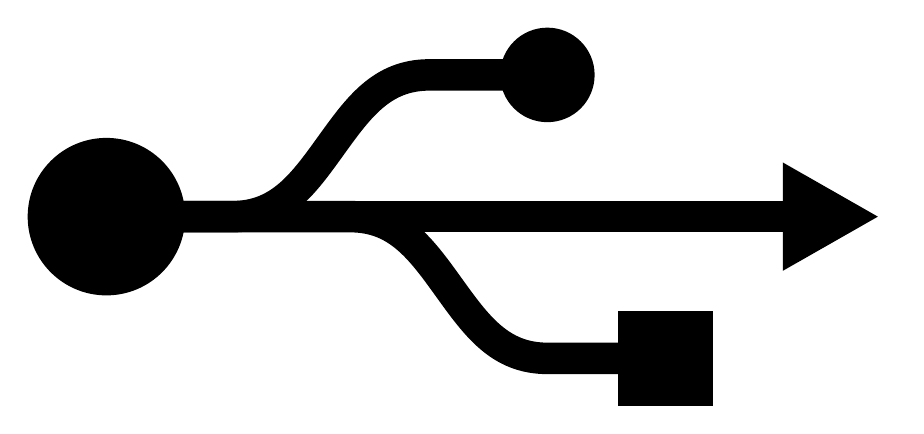
\begin{tikzpicture}[scale=\scl]
        \node [circle, minimum size=\scl*20mm, fill, inner sep=0pt] (start) at (0,0) {};
        \draw[line width=\scl*4mm, {-Stealth[scale=\scl, inset=0pt, length=12.3mm, angle'=55]}]
            (start.center) -- ++(9.82,0)
        ;
        \draw[line width=\scl*4mm, {-Circle[scale=\scl, length=12mm]}]
            (start.center) -- ++(1.6,0) to[out=0, in=234.2461] ++(1.25,0.9) to[out=54.2461, in=180] ++(1.25,0.9) -- ++(2.1,0)
        ;
        \draw[line width=\scl*4mm, {-Square[scale=\scl, length=12mm]}]
            (start.center) -- ++(3.1,0) to[out=0, in=-234.2461] ++(1.25,-0.9) to[out=-54.2461, in=180] ++(1.25,-0.9) -- ++(2.1,0)
        ;
    \end{tikzpicture}
\end{document}
